% % LLNCS macro package for Springer Computer Science proceedings;
% Version 2.21 of 2022/01/12
%
\documentclass[runningheads]{llncs}
%
\usepackage[T1]{fontenc}
% T1 fonts will be used to generate the final print and online PDFs,
% so please use T1 fonts in your manuscript whenever possible.
% Other font encondings may result in incorrect characters.
%

\usepackage{amsmath}
\usepackage{todonotes}
\usepackage{pdfpages}
\usepackage{needspace}

\usepackage[left=2cm,
            right=2cm,
            top=2cm,
            bottom=2cm]{geometry}

\usepackage{graphicx, color, float, subfig}
\captionsetup{font=small,labelfont=bf,labelsep=period,skip=5pt}
\captionsetup[subfloat]{font=scriptsize,labelfont=bf,skip=5pt}

%
\usepackage{hyperref}
\renewcommand\UrlFont{\color{blue}\rmfamily}
\urlstyle{rm}
%

\begin{document}
\title{\fontsize{12}{12}\selectfont Project 2 - Emotion}
\titlerunning{Project 2}
%
\author{Henrik Daniel Christensen\orcidID{hench13@student.sdu.dk} \\Frode Engtoft Johansen\orcidID{fjoha21@student.sdu.dk}}
\authorrunning{Christensen, Johansen} % first names are abbreviated in the running head.
%
\institute{DM873: Deep Learning\\University of Southern Denmark, SDU\\\textit{Department of Mathematics and Computer Science}}
%
\maketitle % typeset the header of the contribution

%%%%%%%%%%%%%%%%%%%%%%%%%%%%%%%%%%%%%%%%%%%
\section{Introduction}
The aim of this project is to design and implement two deep learning models for text/sentiment classification, capable of identifying the emotion conveyed in a given text. The model is trained on the \textit{dair-ai/emotion} dataset, a widely used collection of 20,000 labeled tweets available through Hugging Face. This dataset is divided into six emotion categories: sadness (0), joy (1), love (2), anger (3), fear (4), and surprise (5). Of the total dataset, 2,000 tweets are reserved exclusively for final testing.
\section{Label Distribution}
We started by analyzing the distribution of the labels in the dataset. The distribution of the labels is shown in Figure \ref{fig:label_dist}.
\begin{figure}[H]
    \vspace*{0.7cm}
    \centering
    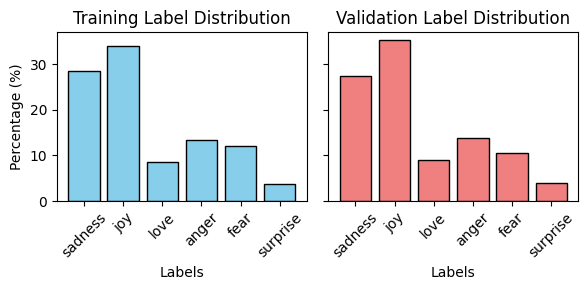
\includegraphics[width=0.22\textwidth]{figures/label_dist.png}
    \caption{Distribution of the labels in the dataset.}
    \label{fig:label_dist}
    \vspace*{0.7cm}
\end{figure}
As can be seen, the dataset is very unbalanced, with the majority of the tweets being labeled as joy or sadness. This could potentially lead to the model being biased towards these labels.
\section{Tokenizing and Vocabulary}
Next, we tokenize the text data for that we created a custom RegexpTokenizer which tokenizes the text by only allowing words, numbers and some special characters. Even though the dataset is rather cleaned. We choose to keep exclamation marks and question marks as they potentially could add value for sentiment analysis.

Next, we check the top 10 most common words in the dataset. First of all, many stopwords are present in the dataset, these could add some value for sentiment analysis, but we expect them to be more noise than signal. Therefore, we remove the stopwords from the dataset. In addition, many words having similar meanings, e.g. 'feel' and 'feeling' are present, therefore these are also removed by stemming the words.

After text cleaning, we could visualize the common words in the sentences by using a WordCloud, see Figure \ref{fig:wordcloud}.
\begin{figure}[H]
    \vspace*{0.7cm}
    \centering
    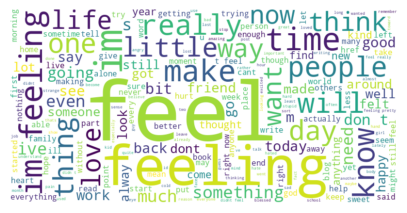
\includegraphics[width=0.4\textwidth]{figures/wordcloud.png}
    \caption{WordCloud of the vocabulary.}
    \label{fig:wordcloud}
    \vspace*{0.7cm}
\end{figure}
As expected many emotional words are present in the vocabulary, e.g. 'love', 'friend', 'hate', 'never', 'go', etc. 

To be able to process the text data, we need to choose a maximum sentence length. A boxplot of the distribution of the lengths of the sequences can be seen in Figure \ref{fig:sequence_length}.
\begin{figure}[H]
    \vspace*{0.7cm}
    \centering
    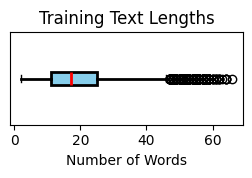
\includegraphics[width=0.22\textwidth]{figures/sentence_length.png}
    \caption{Distribution of the lengths of the sequences.}
    \label{fig:sequence_length}
    \vspace*{0.7cm}
\end{figure}
From the boxplot, we see that the majority of the sequences have a length of around 8 words. We choose to set the maximum sequence length to 10 words. This means that all sequences longer than 10 words are truncated, and all sequences shorter than 23 words are padded with a special token, '<PAD>', to make them all the same length. In addition, we discovered that some sentences are very short, therefore we choose to remove all sentences with a length less than 3 words.

Having our cleaned and tokenized text data, we build a vocabulary from the training dataset. The vocabulary is built by mapping each unique word to an integer. The vocabulary for the training dataset ended up being 10,336 words.

Then, we convert the text data to integers by mapping each word in the text data to the corresponding integer in the vocabulary and pad the sequences to the maximum sequence length. This is done for both the training, validation and test datasets. The text data is now ready to be used for a model.
\section{Models}
Two different models were developed for the sentiment analysis task. The first model is a Recurrent Neural Network (RNN) with Long Short-Term Memory (LSTM) cells, and the second model is a Transformer model.

\subsection{Model 1: RNN-LSTM}
\subsubsection{Model Architecture}
We chose to begin with a Recurrent Neural Network (RNN) model using LSTM (Long Short-Term Memory) cells due to their proven effectiveness in capturing long-term dependencies in sequential data, such as text. LSTMs are particularly suited for this task because they address the vanishing gradient problem often encountered in standard RNNs.

The architecture of the model, shown in Table \ref{tab:rnn_lstm_model}, was designed to balance complexity and performance, resulting in a total of 1,117,734 trainable parameters. Key considerations behind the design are as follows:
\begin{itemize}
    \item Embedding Layer: The vocabulary size of 10,336 and embedding dimension of 75 were chosen to compactly represent the input text while capturing semantic relationships between words effectively. This dimensionality ensures the embeddings are rich enough for the sentiment classification task without being computationally excessive.
          - LSTM Layer: A single LSTM layer with 256 hidden units was selected to provide sufficient capacity to capture sequential patterns in the text. This configuration was chosen to avoid overfitting while retaining the ability to model complex dependencies in the data.
          - Dropout Layer: A dropout rate of 50\% was applied to the LSTM outputs to reduce the risk of overfitting by preventing the model from becoming overly reliant on specific neurons. This regularization technique ensures better generalization to unseen data.
          - Output Layer: The final linear layer maps the 256 features to the 6 output classes, corresponding to the emotions in the dataset.
\end{itemize}

The specific parameters mentioned above was found using a combination of empirical testing (grid search) and theoretical considerations to achieve a balance between model complexity and performance.

\subsubsection{Training and Evaluation}
The model training was conducted using the AdamW optimizer with a learning rate of 0.001 and a batch size of 16. AdamW was chosen due to its effectiveness in handling sparse gradients and its built-in weight decay mechanism, which helps prevent overfitting. The batch size of 16 strikes a balance between computational efficiency and the stability of gradient updates.

For the loss function, we used CrossEntropyLoss, which is well-suited for multi-class classification problems like this one, where the task involves predicting one of six emotion categories. To further regularize the model and reduce the risk of overfitting, an L2-norm penalty (weight decay) of 0.0001 was applied to the weights, encouraging smaller parameter values and promoting a simpler model. The model was trained for 4 epochs, as using more epochs lead to overfitting. The final test accuracy and F1-score is summarized in Table \ref{tab:rnn_lstm_model}.
\begin{figure}[H]
    \vspace*{0.7cm}
    \centering
    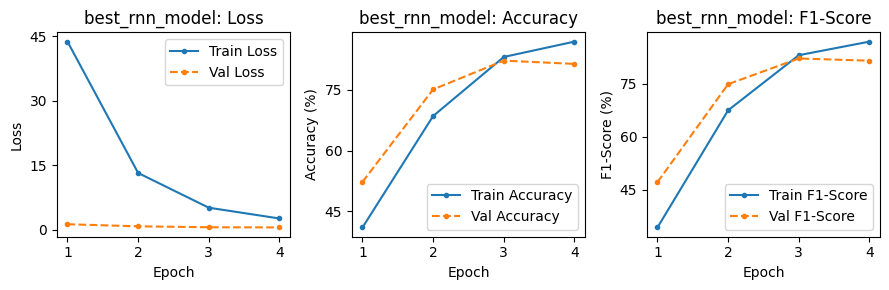
\includegraphics[width=0.6\textwidth]{figures/rnn_scores.png}
    \caption{Training and validation loss, accuracy, and F1-score for the RNN-LSTM model.}
    \label{fig:rnn_scores}
    \vspace*{0.7cm}
\end{figure}

\begin{table}[H]
    \vspace*{-0.5cm}
    \centering
    \begin{tabular}{|l|c|c|c|}
        \hline
        Label        & Precision & Recall & F1-Score \\ \hline
        sadness      & 0.91      & 0.86   & 0.89     \\ \hline
        joy          & 0.85      & 0.86   & 0.85     \\ \hline
        love         & 0.62      & 0.69   & 0.65     \\ \hline
        anger        & 0.84      & 0.81   & 0.82     \\ \hline
        fear         & 0.81      & 0.85   & 0.83     \\ \hline
        surprise     & 0.65      & 0.65   & 0.65     \\ \hline\hline
        accuracy     &           &        & 0.83     \\ \hline
        weighted avg & 0.84      & 0.83   & 0.83     \\ \hline
    \end{tabular}
    \caption{RNN-LSTM model performance on test set.}
    \label{tab:rnn_lstm_model_test}
    \vspace*{-0.8cm}
\end{table}

From the above table, we can see that the model performs well on sadness, joy, anger and fear, but not as well on love and surprise. This is likely due to the imbalanced distribution of the classes in the dataset as discussed in Section \ref{sec:label_distribution}, see Figure \ref{fig:label_dist}.
\subsection{Model 2: Transformer}
The model is made from the solution to exercise sheet 5. Very few elements have been changed since it follows the pages in the Bishop book closely. The only big changes that has been made to the model itself is added dropout layers and positional encoding. We also experimented with randomly removing 2 tokens from each sentence to increase generalisation but it didn't work. WE also tried adding 2 more linear layers to the transformer block, but this was detrimental to the accuracy so we removed them again.
We chose to use a transformer model as it seems like a good architecture for working with text since it makes words weigh differently depending on which other words are present in the sentence, and with positional encoding also where they are in that sentence. This is important since the meaning of words change depending on other words, and position in sentence.
We used sinusoidal position embedding since this is the positional embedding used in the Bishop book.
The L in the sinusoidal position embedding is 10000. The example in the Bishop book had an L of 30, and some other examples we encountered had an L of 10000. We chose 10000 as the value for L since we encountered it multiple places.\\

We used cross entropy loss as a our loss function since this is a good loss function for classification tasks.
This is the number of heads in the multi head self attention mechanism. d\_model should preferably be divisible by this number so each head computes the same size of input. We chose 8 heads since having too many heads can be inefficient and since we have d\_model of 128, choosing more heads would lead to quite few dimensions per head, which would make it hard for them to capture any useful features.
The mlp factor controls the amount of nodes in the linear layers of the transformer block. We use an mlp factor of 4. This was the default value and decreasing this value hit the performance of the model. Increasing the mlp factor would increase the training time so we decided to not do that.
d\_model is the dimensions of each token. We have a vocabulary of 10336 so we made this pretty big to ensure that each word is able to be uniquely represented. \\

We have 6 layers of transformer blocks. According to the slides, 6 layers is a normal amount of layers and 12 layers is for very large models. We experimented with 6 and 12 layers and found only a small performance increase with 12 layers, but a significant increase in training time, so we decided that we would rather train quicker to test values for other parameters.
When training the transformer models with different parameters we found out that they would quickly overfit, so we needed to generalise the model. To do this we added two dropout layers on the linear layers of the transformer blocks. The dropout chance for the first layer is 50\% and for the second layer is 25\%. We tested with both higher and lower dropout chances and this worked the best.
We chose adam as the optimizer. From the last project our and other peoples takeaway were that adam was a good optimizer in general, and since were not using weight decay, we don't need to use adamW.
We used a learning rate of 0,0003. This was discussed as a good learning rate from the last project, and our experimenting also led us to this learning rate.
We experimented a bit with using weight decay but it did not work well so we decided not to use it in our final model.
When testing different parameters, we used 50 epochs. The transformer models quickly overfitted so we didn't need more epochs. 
We experimented with both L1 and L2 regularisation. L1 regularisation worked the best, and that is probably because it makes some weights go to 0, which indicates those words aren't important. In sentences, some words tells more than other words, so it makes sense that this would be good.

\begin{figure}[H]
    \vspace*{0.7cm}
    \centering
    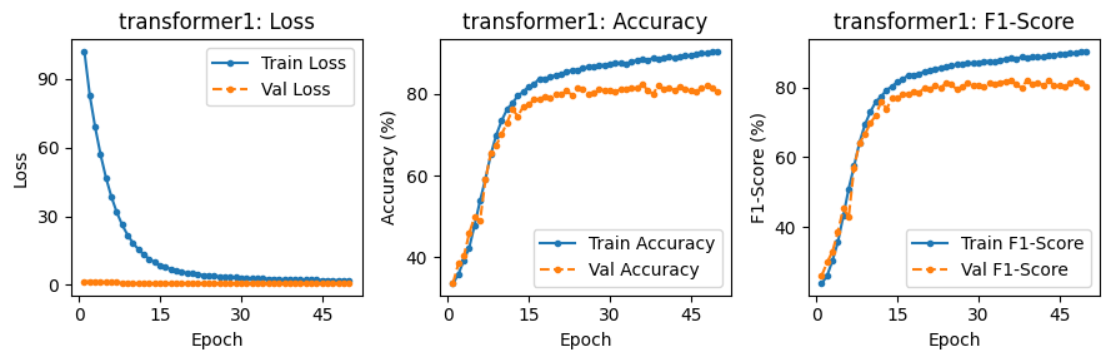
\includegraphics[width=0.6\textwidth]{figures/transformer_scores.png}
    \caption{Training and validation loss, accuracy, and F1-score for the transformer model.}
    \label{fig:transformer_scores}
    \vspace*{0.7cm}
\end{figure}

\begin{table}[H]
    \vspace*{-0.5cm}
    \centering
    \begin{tabular}{|l|c|c|c|}
        \hline
        Label        & Precision & Recall & F1-Score \\ \hline
        sadness      & 0.89      & 0.82   & 0.85     \\ \hline
        joy          & 0.81      & 0.88   & 0.85     \\ \hline
        love         & 0.68      & 0.59   & 0.63     \\ \hline
        anger        & 0.77      & 0.81   & 0.79     \\ \hline
        fear         & 0.80      & 0.80   & 0.80     \\ \hline
        surprise     & 0.67      & 0.56   & 0.61     \\ \hline\hline
        accuracy     &           &        & 0.81     \\ \hline
        weighted avg & 0.81      & 0.81   & 0.81     \\ \hline
    \end{tabular}
    \caption{Transformer model performance on test set.}
    \label{tab:rnn_lstm_model_test}
    \vspace*{-0.8cm}
\end{table}

Despite a lot of parameter tuning, we could not get the transformer model to get a better performance. We even tried adding extra linear layers in the transformer block, and removing random words from the sentences for better generalisation.

\section{Analysis and Final Prediction}
% The reg\_4 model is now applied to the test set to evaluate its performance. The test accuracy is summarized in Table \ref{tab:prediction}.

% \begin{table}[H]
%     \centering
%     \begin{tabular}{|c|c|}
%         \hline
%         \textbf{Test Accuracy using Reg4 model} \\ \hline
%         91.5\% \\ \hline
%     \end{tabular}
%     \caption{Test Accuracy using Reg4 Model.}
%     \label{tab:prediction}
% \end{table}

% Some of the misclassified and correctly classified images are given in Figure \ref{fig:prediction}.
% \begin{figure}[H]
%     \vspace*{-0.7cm}
%     \centering
%     \includegraphics[width=1\textwidth]{figures/predict_images.png}
%     \caption{Misclassified and correctly classified images.}
%     \label{fig:prediction}
%     \vspace*{-0.7cm}
% \end{figure}

% From the misclassified images, we see that may some more data augmentation could be applied to improve the model's performance. For example, the cat that rotate its head by almost 90 degrees. Moreover, the model may be improved by adding more crop-scale augmentation.
\section{Pretrained Model (DistilBERT)}
To evaluate how our model compares to a larger pretrained model, we utilized the DistilBERT base model (uncased) from Hugging Face. DistilBERT is a distilled version of BERT, pretrained on a large corpus comprising 11,038 books and the English Wikipedia. It features a vocabulary size of 30,000 tokens and contains approximately 67 million parameters, making it significantly larger and more complex than our models. To adapt DistilBERT to our sentiment analysis task, we fine-tuned the model for 5 epochs using a small initial learning rate of $5\times10^{-6}$. This low learning rate ensures stable and effective fine-tuning of the pretrained weights without overfitting to our dataset. The performance of DistilBERT on our task is summarized in Table \ref{tab:distilbert_model}.

\begin{table}[H]
    \vspace*{-0.5cm}
    \centering
    \begin{tabular}{|l|c|c|c|}
        \hline
        Label        & Precision & Recall & F1-Score \\ \hline
        sadness      & 0.92      & 0.93   & 0.92     \\ \hline
        joy          & 0.90      & 0.92   & 0.91     \\ \hline
        love         & 0.74      & 0.71   & 0.72     \\ \hline
        anger        & 0.90      & 0.89   & 0.89     \\ \hline
        fear         & 0.87      & 0.89   & 0.88     \\ \hline
        surprise     & 0.82      & 0.61   & 0.70     \\ \hline\hline
        accuracy     &           &        & 0.89     \\ \hline
        weighted avg & 0.89      & 0.89   & 0.89     \\ \hline
    \end{tabular}
    \caption{DistilBERT model performance on test set.}
    \label{tab:distilbert_model}
    \vspace*{-0.8cm}
\end{table}

From the above results, we see that the pretrained model performs generally better than our two models. Notice that the performance on the less presents classes love and surprise is also lower as seen in the previous models.
\section{Conclusion}
We constructed two different models to complete the task, a recurrent neural network with LSTM and 256 hidden units, and a transformer model with 6 transformer layers. The recurrent neural network had the best test accuracy of 83\%, while the transformer model had a test accuracy of 81\%. We tried using a pretrained model distilBERT on our task to see how it would fare. It got a test accuracy of 89\%. As expected our models were worse. This can be explained by the fact that distilBERT has more parameters and a much bigger training set than our models. 

Overall we are satisfied with our result but it could have been improved. Initially an accuracy of 83\% seems quite bad, but even the pretrained model had a test accuracy of less than 90\% so compared to that, it does not seem too bad. 

\subsection{Individual Contributions}
\begin{table}[H]
    \centering
    \begin{tabular}{|l|l|l|}
    \hline
                    & \textbf{Henrik Daniel Christensen}    & \textbf{Frode Engtoft Johansen} \\ \hline
    \textbf{Code}   & Task 1, 2, 5                          & Task 3, 4\\ \hline
    \textbf{Report} & Section 1, 2, 3, 4.1, 6                 & Section 4.2, 5, 7 \\ \hline
    \end{tabular}
    \caption{Individual contributions.}
    \label{tab:individual_contributions}
\end{table}


%%%%%%%%%%%%%%%%%%%%%%%%%%%%%%%%%%%%%%%%%%%

%Appendices
\newpage
\appendix
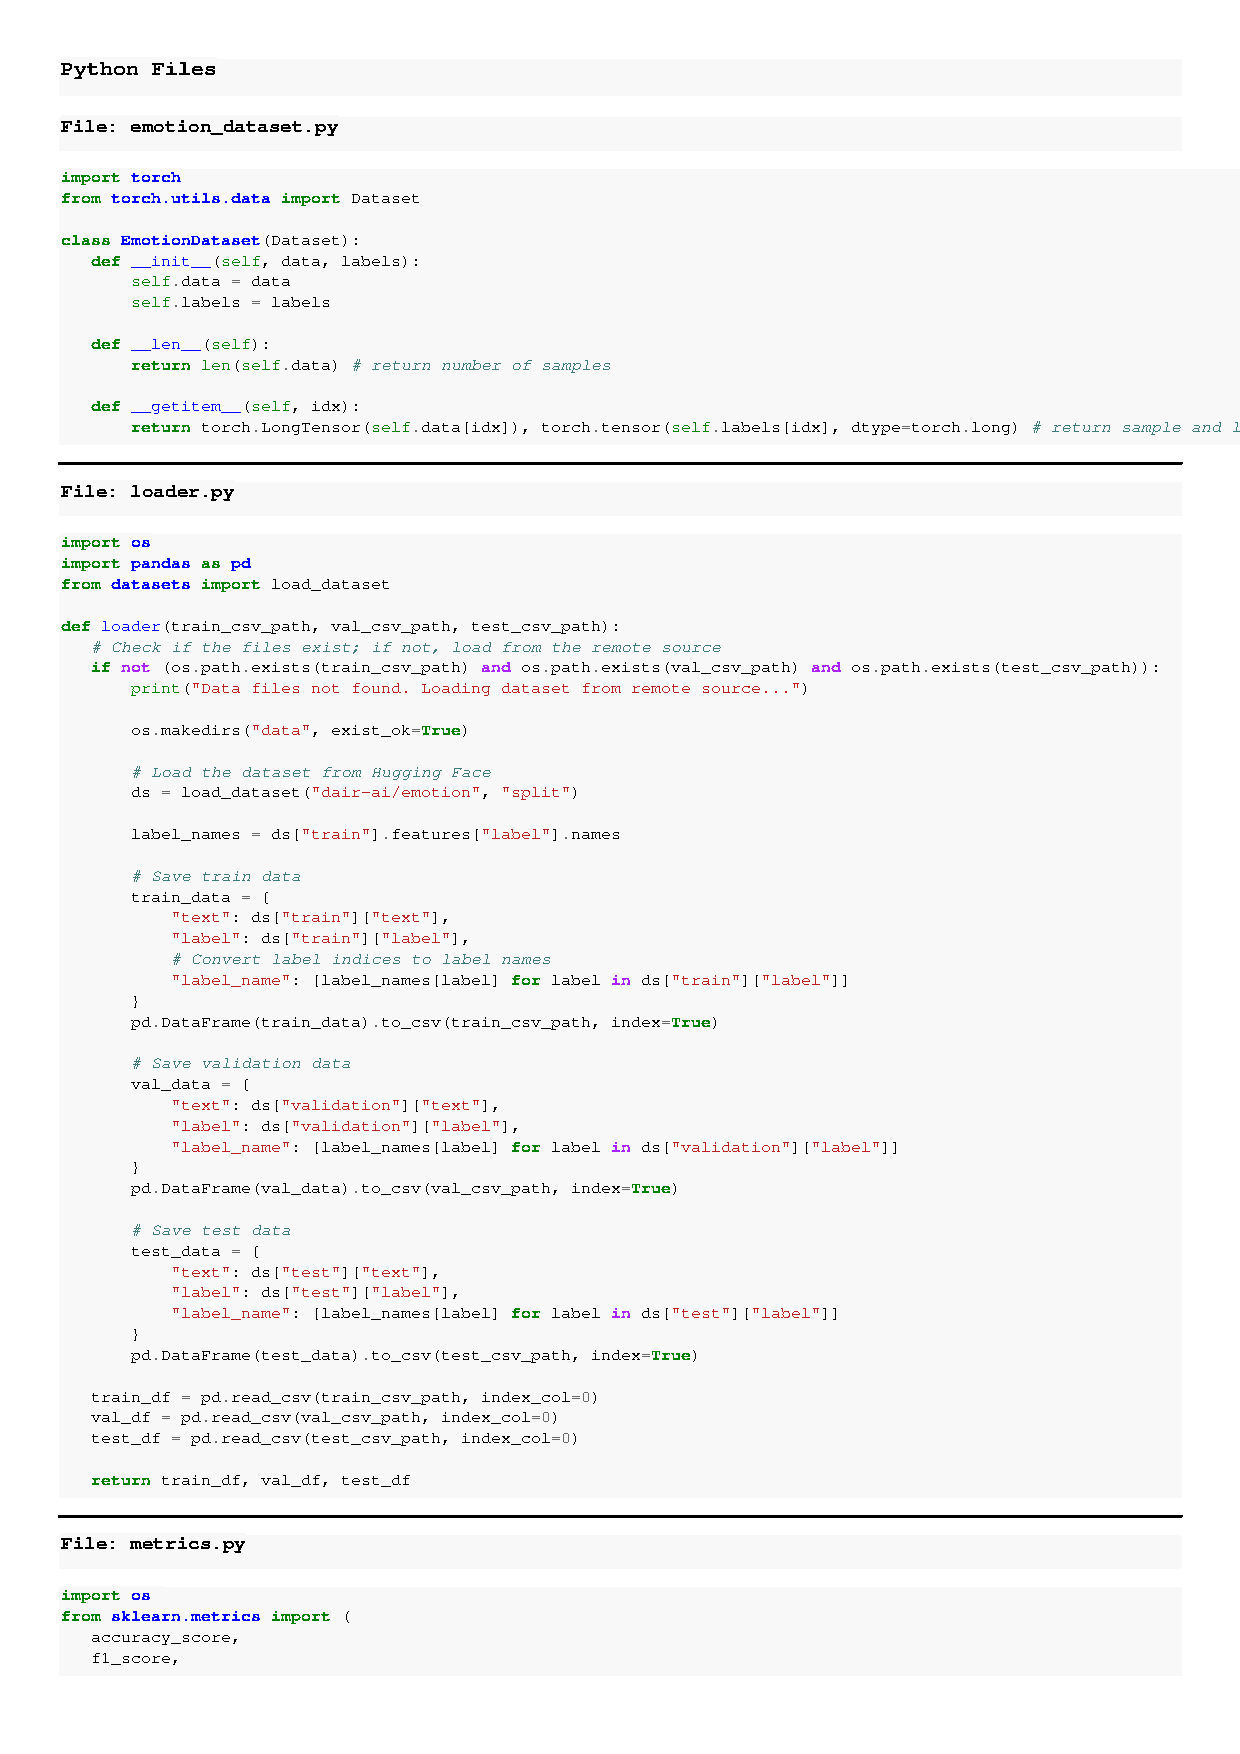
\includepdf[pages=1,scale=.85,pagecommand={\section{Code}\label{app:code}}]{../src/code.pdf}
\includepdf[pages=2-,scale=.85,pagecommand={}]{../src/code.pdf}
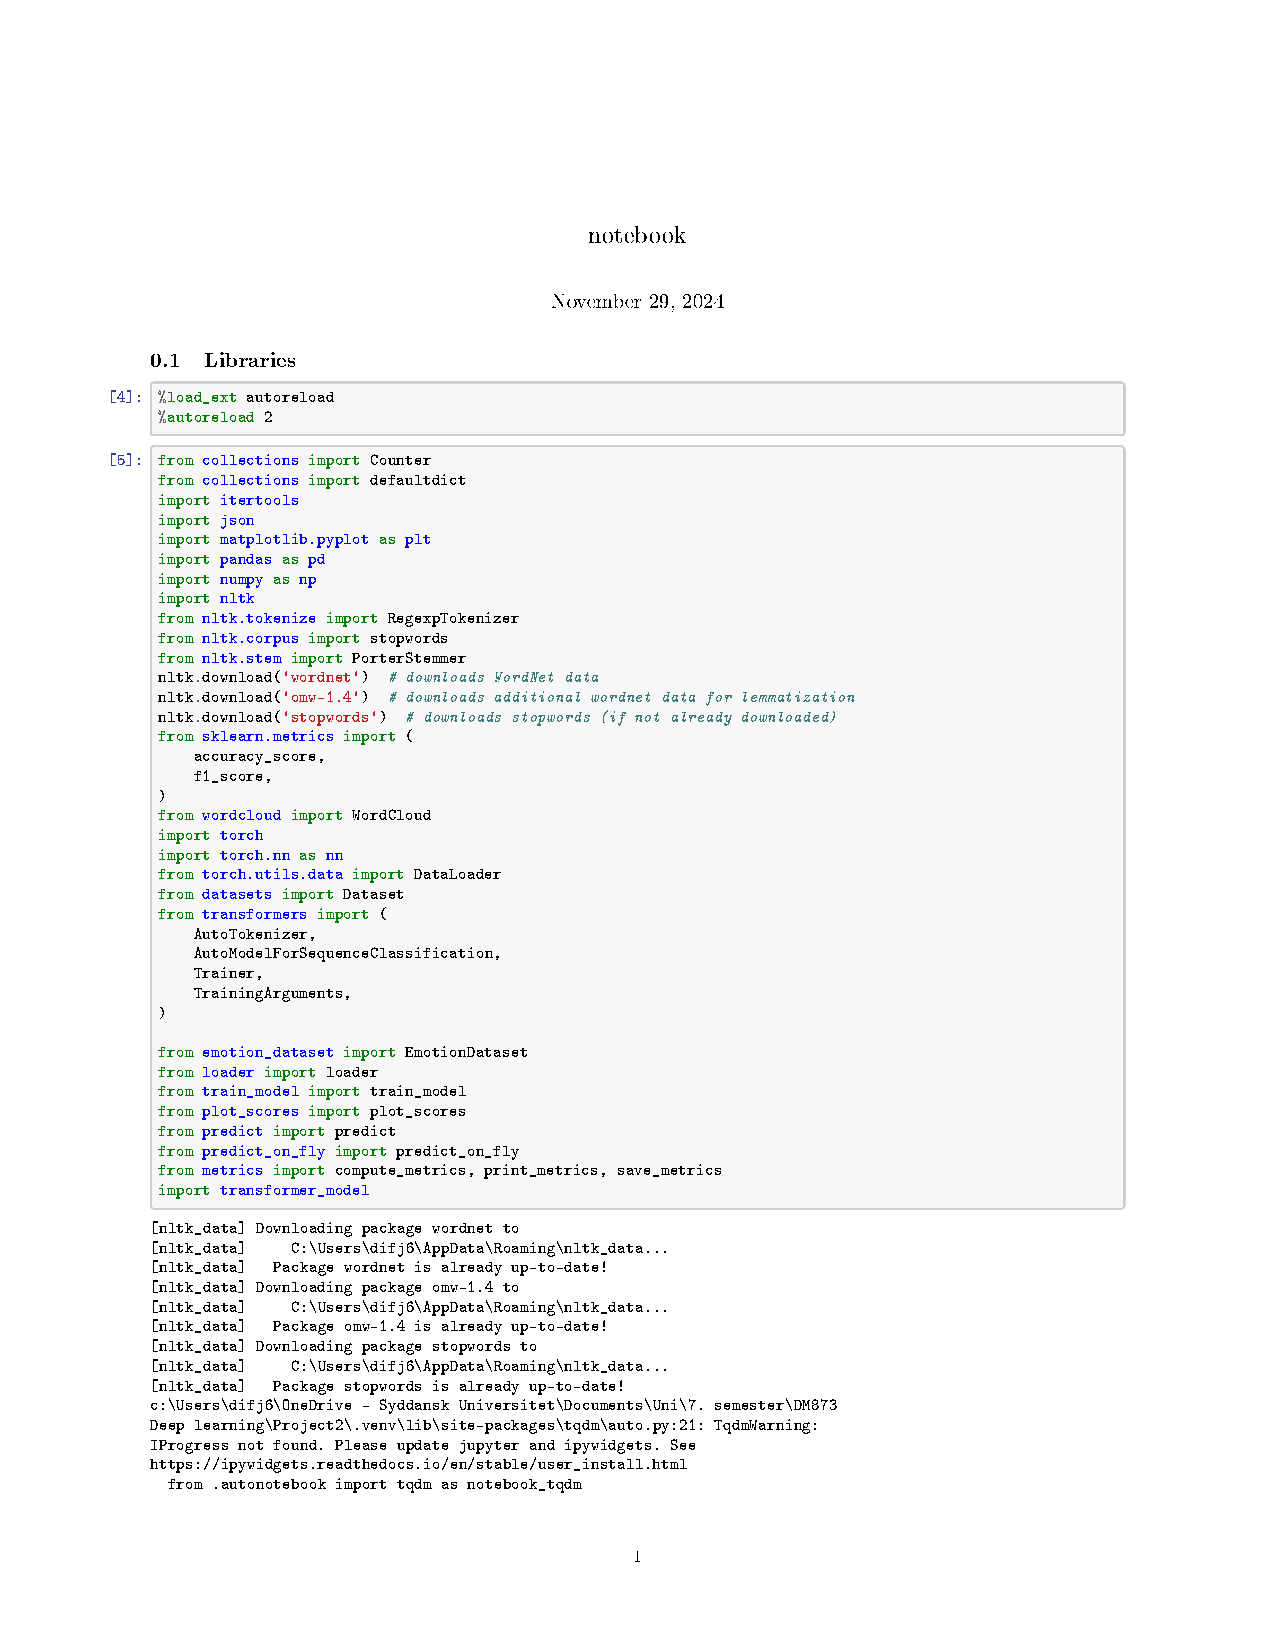
\includepdf[pages=1,scale=.85,pagecommand={\section{Notebook}\label{app:notebook}}]{../src/notebook.pdf}
\includepdf[pages=2-,scale=.85,pagecommand={}]{../src/notebook.pdf}

% \bibliographystyle{base/splncs04}
% \newpage
% \bibliography{base/references}
%%%%%%%%%%%%%%%%%%%%%%%%%%%%%%%%%%%%%%%%%%%
\end{document}